\section{Runtime Libraries}\label{sec:runtime}

The layer of the runtime libraries are shown in \fig{layer}.
One of the three underlying communication libraries is selected 
at the build time of the Omni compiler.
The coarray runtime consists of layered three libraries.
\begin{itemize}
\item
The {\bf lower-level runtime library (LRL)} abstracts the difference between 
the communication libraries except the memory management of coarray data.
\item
The {\bf upper-level runtime library (URL)} solves each coarray features 
in the coarray program.
\item
The {\bf Fortran wrapper} mediates the arguments and the result value 
of the translated user program (written in Fortran) and URL (written in C).
\end{itemize}


\begin{figure}[tbh]
  \begin{center}
    % trimはleft bottom right topの順
    %\mbox{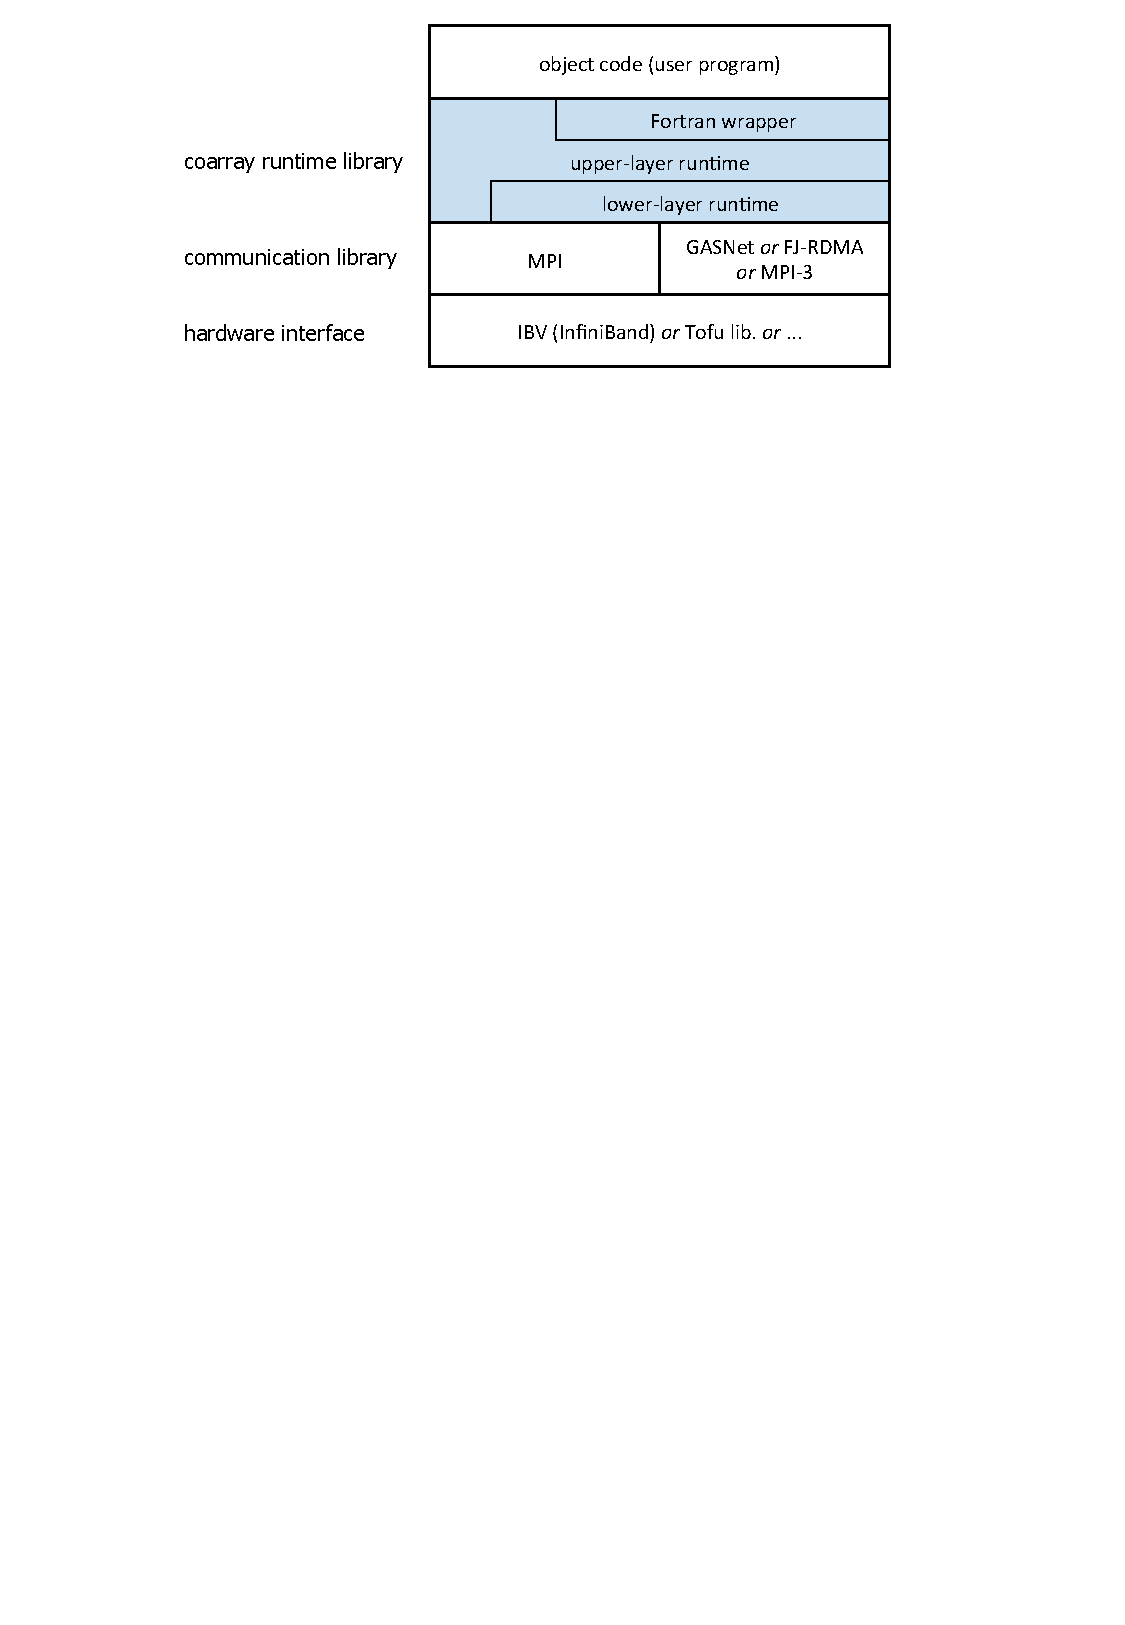
\includegraphics[trim=42mm 210mm 47mm 0mm, scale=0.7,clip]{figs/softstack-r2.pdf}}
    \mbox{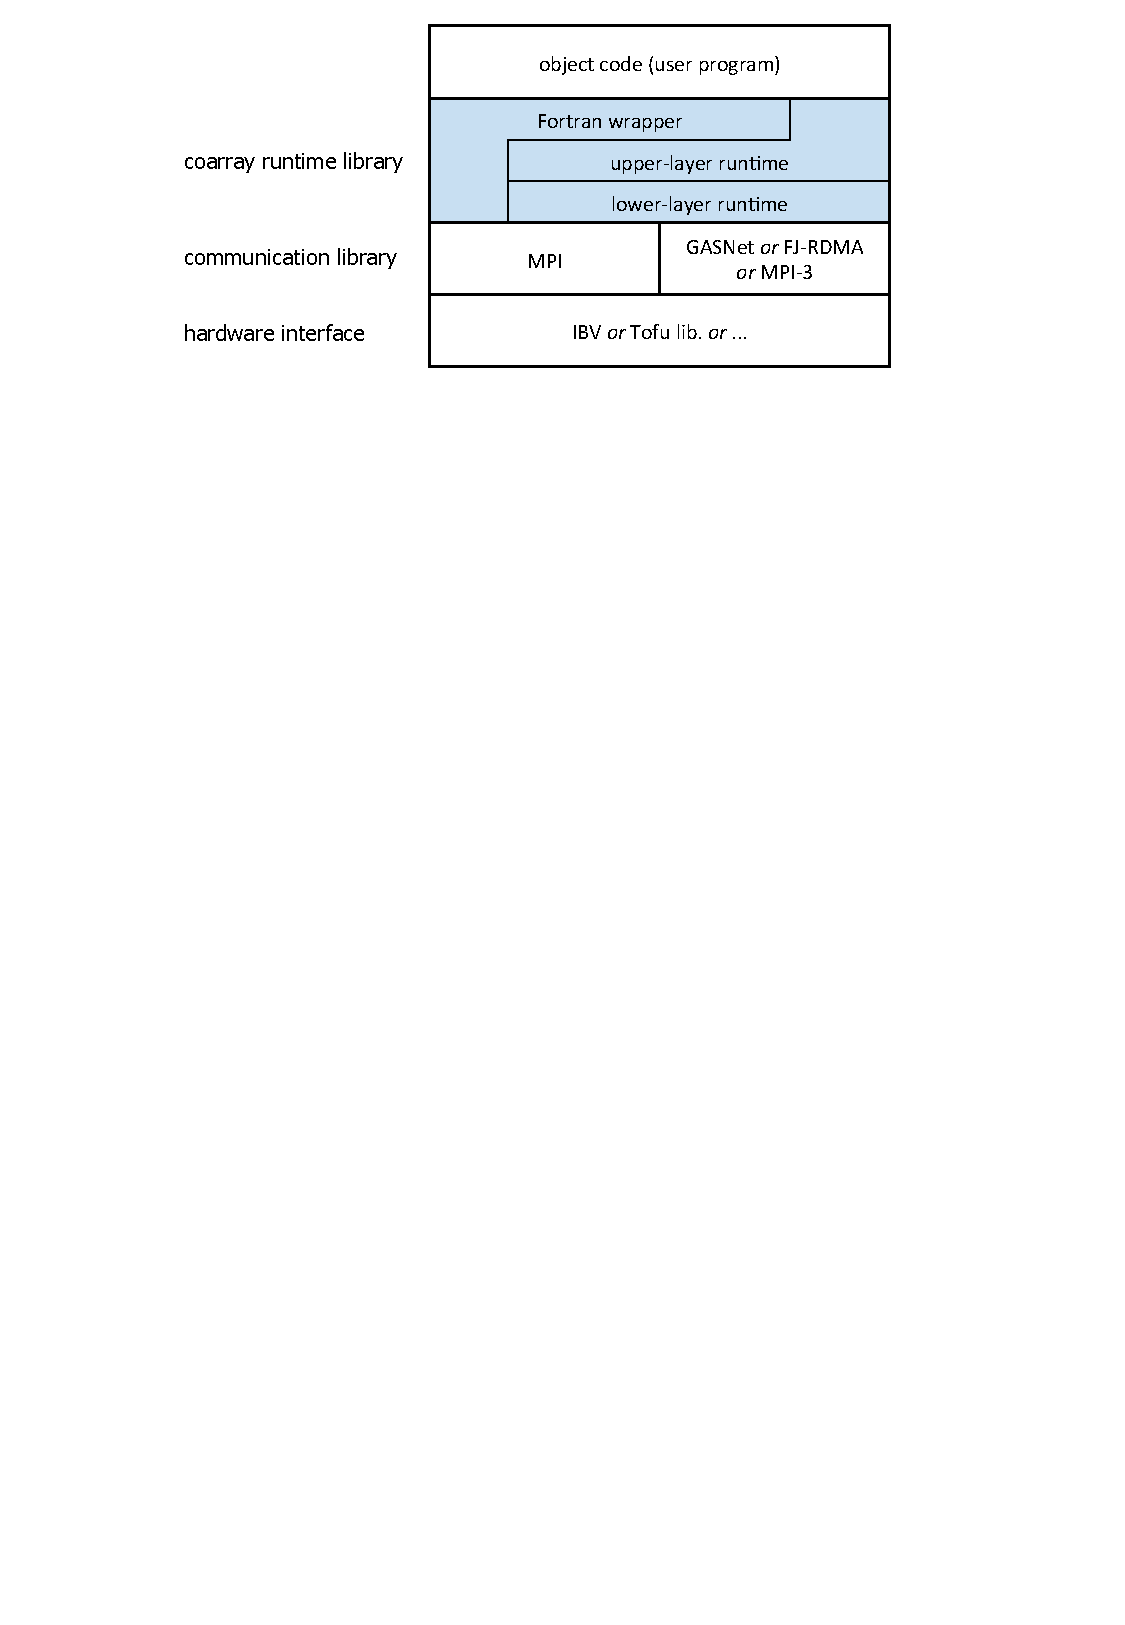
\includegraphics[trim=27mm 208mm 29mm 0mm, scale=0.7,clip]{figs/softstack-r4.pdf}}
    \caption{Software stack for coarray features}\label{fig:layer}
  \end{center}
\end{figure}


%-----------------------------------------------------------------------------
\subsection{Underlying Communication libraries}
%-----------------------------------------------------------------------------

MPI-3 can be selected for all platform on which MPI-3 is implemented. Coarrays are 
registered and deregistered at the start and end point of the MPI window. 
Coarrays are performed one-sided communication by {\tt MPI\_Put} and {\tt MPI\_Get},
and synchronized by {\tt MPI\_Win\_fence}. 
Implementation on MPI incurs certain costs for dynamic allocation of coarrays and 
waiting for communication completion.

GASNet can be selected for more advanced implementation over InfiniBand. 
Since allocation and registration of are inseparable and can be done only once 
on GASNet, the implementation allocates and registers a pool of memory
whose size should be large enough to contain all static and allocatable coarrays.
The XMP runtime should allocate and deallocate coarrays not using the Fortran 
library but using the memory manager made for the pool.

FJ-RDMA can be selected for the implementation over Tofu interconnect of 
the K computer and Fujitsu PRIMEHPC FX series supercomputers. 
Basically, each coarray is allocated by the Fortran library and registered 
the address with the FJ-RDMA interface {\tt FJMPI\_Rdma\_reg\_mem}. 
And it is deregistered with {\tt FJMPI\_Rdma\_dereg\_mem} before deallocated 
(freed) by the Fortran library. 
One-sided communication is performed with {\tt FJMPI\_Rdma\_put} and 
{\tt FJMPI\_Rdma\_get}.
%, which include confirmation of communication completion. <-- 本当? いつも?


%-----------------------------------------------------------------------------
\subsection{Lower-layer runtime library (LRL)}
%-----------------------------------------------------------------------------

LRL abstracts the difference between the communication libraries except 
which allocates the coarray data between the coarray runtime 
(by the RS and RA methods) and the Fortran system (by the CA method).
The features for multi-dimensional data developped for the C implementation
are not used for the Fortran implementation.

The LRL functions currently used in the Fortran implementation are as follows.
\begin{itemize}
\item
A set of functions to allocate and register a specified size of coarray,
and a set of functions to register an already-allocated coarray.
They are alternatively used in the RS and RA methods and in the CA method.
Corresponding to each, a set of functions to deregister and deallocate and
a set of functions to deregister are provided.

\item
A function for RDMA-DMA GET communication with specified-length contiguous
data, and the one of DMA-RDMA PUT communication.
They assume that both remote and local data are previously registered.
Blocking and non-blocking can be switched and the only way to wait for
the completion of the non-blocking communication is using the function
corresponding to {\tt SYNC MEMORY}.

\item
Functions corresponding to the {\tt SYNC ALL}, {\tt SYNC IMAGES} and 
{\tt SYNC MEMORY} statements. 
The function corresponding to {\tt SYNC MEMORY} waits for completion of all 
current non-blocking communications.

\item
Functions corresponding to the {\tt ATOMIC\_DEFINE} and {\tt ATOMIC\_REF} 
intrinsic subroutines. Each has two versions for self and remote images.
Unlike PUT/GET functions, they always work in blocing.

\item
Some inquire functions.
\end{itemize}

% \hline
% 割付け・解放と登録
% & 1. \verb|_XMP_coarray_malloc_image_info_1|\\
% & 2. \verb|_XMP_coarray_malloc_info_1|\\
% & 3. \verb|_XMP_coarray_malloc_do|\\
% & 4. \verb|_XMP_coarray_regmem_do|\\
% & 5. \verb|_XMP_coarray_lastly_deallocate|\\
% \hline
% 片側通信
% & 6. \verb|_XMP_coarray_shortcut_get|\\
% & 7. \verb|_XMP_coarray_shortcut_put|\\
% \hline
% 同期
% & 8. \verb|xmp_sync_all|\\
% & 9. \verb|xmp_sync_image|\\
% & 10 \verb|.xmp_sync_images|\\
% & 11 \verb|.xmp_sync_images_all|\\
% & 12 \verb|.xmp_sync_memory|\\
% \hline
% atomic通信
% & 13 \verb|._XMP_atomic_define_0|\\
% & 14 \verb|._XMP_atomic_define_1|\\
% & 15 \verb|._XMP_atomic_ref_0|\\
% & 16 \verb|._XMP_atomic_ref_1|\\
% \hline
% 問合せ
% & 17 \verb|.xmp_all_num_nodes|\\
% \hline
% エラー処理
% & 18 \verb|._XMP_fatal|\\
% \hline
%   \end{tabular}
%  \end{center}
% \end{table}


%-----------------------------------------------------------------------------
\subsection{Upper-layer runtime library (URL)}
%-----------------------------------------------------------------------------

URL implements three kinds of coarray communications as follows:
\begin{itemize}
\item
For one-sided PUT/GET communications caused by the referrence of coindexed
variables/objects, the algorithm shown in \Sec{putget} is implemented in URL. 
The algorithm requires only the contiguous communicaton between 
pre-registered local and remote data.
The Fortran wrapper mediates the argument interfaces.

\item 
For collective commnications caused by intrinsic subroutines 
{\tt CO\_SUM}, {\tt CO\_MAX}, {\tt CO\_MIN} and {\tt CO\_BROADCAST}, 
URL lost the role in the latest implementation. 
The Fortran wrapper uses MPI library functions directly.

\item
For atomic communications caused by intrinsic subroutines
{\tt ATOMIC\_DEFINE} and {\tt ATOMIC\_REF}, 
URL calls the corresponding function of LRL after address calculation.
\end{itemize}



%-----------------------------------------------------------------------------
\subsection{Fortran wrapper}
%-----------------------------------------------------------------------------
While the coarray runtime is written in C, coarray features are 
based on array notations specified in Fortran~90 or later.
The Fortran wrapper is a part of the coarray runtime and mediates
Fortran and C argument interfaces.

For example, suppose {\\tt a} is a two-dimensional array coarray of 
16-byte complex type. The value of a coindexed object:
\begin{center}\tt
a(1:10,2:19)[{\it k}]
\end{center}
should be a two-dimensional array shaped {\tt [} 10, 18 {\tt ]}. 
The coarray translator converts it to a wrapper function call:
\begin{center}\tt
xmpf\_coarray\_get\_generic({\it desc\_}a, {\it k}, a(1:10,2:19))
\end{center}
where {\tt{\it desc\_}a} is the descriptor of coarray {\tt a}.
Note that the generic function name is used in the output of the coarray
translator. The corresponding specific name is selected in the 
following Fortran compiler as shown below:
\begin{center}\tt
xmpf\_coarray\_get2d\_z16({\it desc\_}a, {\it k}, a(1:10,2:19))
\end{center}
where {\tt xmpf\_coarray\_get2d\_z16} means the wrapper function
of GET communication for two-dimensional and 16-byte complex type.
The last argument is a mold expression to get the communication pattern 
and the shape of the result value.
At last, this function invokes the C-written runtime function:
\begin{center}\tt
xmpf\_coarray\_get\_array({\it desc\_}a,\,base,\,16,\,{\it k},\,dst,\,2,\,skip,\,extent)
\end{center}
where, 
\begin{itemize}
\item
{\tt base} is the address of {\tt a(1,2)} that is the base address of 
{\tt a(1:10,2:19)},
\item
{\tt dst} is the result variable of 16-byte complex shaped {\tt [} 10, 18 {\tt ]}
in Fortran, or, the pointer to 16 $\times$ 10 $\times$ 80-byte memory in C, and
\item
{\tt skip} and {\tt extent} are two-dimensional integer arrays to represent 
the pattern of the communication data.
\end{itemize}

As shown in this example, the Fortran wrapper solves
multi-dimensional array segments of Fortran into C, and vise visa.
It also converts a C pointer to a Fortran pointer with the shape, using
the Cray pointer and tricky coding.

%Actually, the interface is used through the Fortran~90 generic interface
%to ease the code generation by the coarray translator.
%For example, let us convert an {\tt ALLOCATE} statement
%{\tt allocate (a(1:10,2:19))}, where {\tt a} is an allocatable coarray of 16-byte,
%using object-ULR interface {\tt XMPCO\_malloc\_coarray}.
%The translator may generate a call to the generic procedure \\
%{\tt xmpf_coarray_malloc_generic(descriptor_of_a, a, 


